\chapter{Material and Methods}
\label{ch:methods}

\section{Base Model: UK Biobank-Trained Plaque Detection Model}
\label{sec:base-model}

The starting point for this thesis is a deep learning model for automated detection of
atherosclerotic plaques in carotid ultrasound images, originally developed by
\textcite{omarov2024deep} at the Institute for Stroke and Dementia Research (LMU Munich).

\subsection{Original Training Data and Annotation}
The model was trained on carotid ultrasound images collected during the first imaging visit of
the UK Biobank cohort, following the acquisition protocol and quality-assurance procedure
described by \textcite{coffey2017protocol}. From a pool of 177{,}757 raw images across 19{,}499 participants,
38{,}732 images acquired in the longitudinal axis of the left and right distal common carotid
artery and the bifurcation were retained for analysis, and plaque annotation was performed on a
subset of these. Participants had a mean age of 64.6 years (SD 7.59) at the time of the carotid
ultrasound examination, 50.8\,\% were female, and 1{,}381 (7.1\,\%) had a baseline diagnosis of
atherosclerotic cardiovascular disease. Plaques were manually annotated by trained clinicians in
680 randomly selected images, following standard criteria \cite{touboul2012mannheim} (focal
protrusion into the arterial lumen with a thickness exceeding 50\,\% of the surrounding carotid
intima-media thickness). A plaque was present in 253 of the 680 annotated images.

\subsection{Model Architecture and Training}
\textcite{omarov2024deep} employed a YOLOv8l object detection architecture
\cite{jocher2023ultralytics}, pre-trained on a large corpus of natural images and subsequently
fine-tuned via transfer learning on the annotated carotid ultrasound subset. The annotated data
were split into training, validation, and test sets at a ratio of 0.725/0.125/0.15. To improve
generalizability, roughly half of the training images were augmented using the Albumentations
library \cite{buslaev2020albumentations} (grid distortion, brightness/contrast adjustment,
horizontal flipping, Gaussian noise, and random-sized cropping), in addition to a reduced set of
YOLOv8's built-in augmentations. Loss function weights
(distribution focal loss, box loss, and binary cross-entropy loss) were tuned via grid search,
and training used a batch size of 44 with early stopping. Five-fold cross-validation on the
development set showed consistent performance across folds, indicating limited overfitting.

\subsection{Original Model Performance}
\label{subsec:base-model-performance}
On a held-out test set of 103 images (38 containing at least one plaque), the model achieved
an image-level classification accuracy of 89.3\,\%, sensitivity of 89.5\,\%, specificity of
89.2\,\%, and a positive predictive value of 82.9\,\%, at a confidence threshold of 13\,\%
(Table~\ref{tab:base-model-performance}). The 103 test images contained 53 plaques in total. At
the object-detection level, the model reached a mean average precision at an IoU threshold of
50\,\% (mAP@50) of 68.4\,\%, with a detection precision of 70.3\,\% and a detection recall of
71.7\,\%. Applied to the full cohort, the model identified carotid plaques in 45\,\% of
participants.

The image-level figures (around 89\,\%) and the detection-level ones (around 70\,\%) answer
different questions and are not comparable with one another; Section~\ref{subsec:metrics}
sets out which of the two this thesis reports and why.

\begin{table}[H]
\centering
\caption[Original model performance]{Classification performance of the base model on the
original UK Biobank held-out test set (103 images), as reported by \textcite{omarov2024deep}.}
\label{tab:base-model-performance}
\begin{tabular}{lcccc}
\hline
& Accuracy & Sensitivity & Specificity & PPV \\
\hline
Base model (UK Biobank test set) & 89.3\,\% & 89.5\,\% & 89.2\,\% & 82.9\,\% \\
\hline
\end{tabular}
\end{table}

This baseline performance -- and, in particular, the four false negatives out of 38
plaque-positive test images -- serves as the reference point against which the external
validation and fine-tuning described in Section~\ref{sec:phase2} (Phase 2) of this thesis are
evaluated.

\section{Reproduction of the Detection Pipeline on UK Biobank}
\label{sec:reproduction}

Individual-level results of \textcite{omarov2024deep} cannot be shared directly because of UK
Biobank data-protection and access restrictions. Deriving plaque phenotypes for the analyses in
this thesis therefore required re-running the published pipeline on the UK Biobank Research
Analysis Platform rather than obtaining its outputs. Beyond reproduction, this step was also used
to derive image-level plaque counts (0--3 detections per image), which the original setup does
not provide as a standalone output but which are required downstream.

\subsection{Pipeline Adaptations}
The implementation follows the preprocessing and inference logic of \textcite{omarov2024deep} as
closely as possible. Two adaptations were made to remove manual steps that would not scale to
the full cohort. First, an alternative grey-value filtering approach was used during
preprocessing; the operation is a standard grey-level transform, and the exact step it replaced
was not recorded. Second, the selection of the relevant long-axis
(main-axis) image from each acquisition was automated. Each archive holds several frames, only
some of which show the vessel in the longitudinal plane; that view is the one the plaque
criterion is defined in, because it requires a focal protrusion to be measured against the wall
on either side of it, which a cross-sectional frame does not display.

Main-axis selection exploits a constant signature in the image data. A fixed region of the
device display is rendered identically whenever the long-axis view is active, so the sum of its
pixel values is the same in every such frame and differs in the others. Frames are therefore
matched against a reference value of 980{,}305 rather than ranked by any image property. The
value is an exact-match fingerprint of that display state and carries no meaning beyond
identifying it; it was obtained by reading it off frames known to show the long-axis view.

Matching on an exact sum is deliberate but brittle: it selects the intended frame without a
tolerance parameter, and it fails outright rather than silently returning a wrong frame if the
display state differs at all. Archives in which no frame matched were therefore recorded as
failures and excluded rather than resolved by a fallback rule. Figure~\ref{fig:ukb-pipeline} shows the sequence applied to a single acquisition.

\begin{figure}[H]
\centering
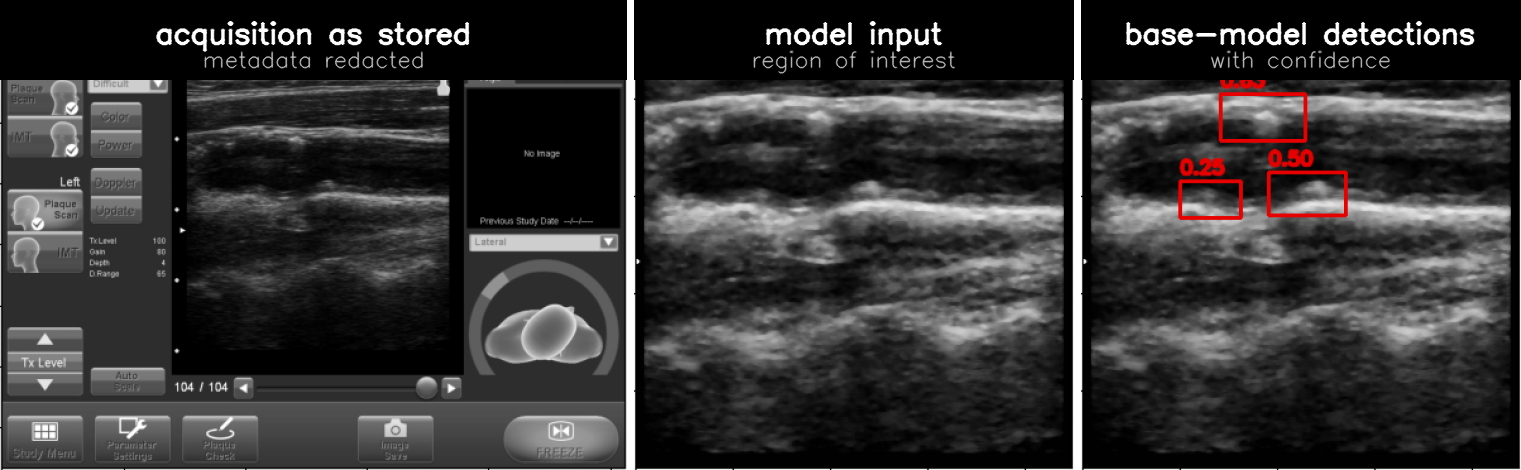
\includegraphics[width=\textwidth]{figures/ukb_pipeline.png}
\caption[The reproduced inference pipeline]{The pipeline applied to one UK Biobank acquisition.
Left: the frame as stored, comprising the full device display; the band carrying participant
identifiers and the acquisition timestamp has been redacted. Centre: the region of interest
extracted and converted to grey-scale, which is what the model receives. Right: the resulting
detections with their confidence scores, at the operating threshold of the published pipeline.}
\label{fig:ukb-pipeline}
\end{figure}

\subsection{Execution Environment}
UK Biobank data may not leave the Research Analysis Platform, so both preprocessing and inference
were executed there rather than locally. The platform provisions cloud compute instances, and
GPU-equipped instances with sufficient memory to hold the extracted image archives were used for
the inference run.
The instance was selected from the platform's mid-range GPU category, described there as
suitable for training smaller models and running machine-learning workflows. The exact
specification was not recorded at the time of the run and the platform's instance catalogue
changes over time, so a reader repeating the work should select by that category rather than by
an instance identifier.

\subsection{Scale of the Reproduction}
\label{subsec:reproduction-scale}
Inference was run over 43{,}636 archives, comprising 179{,}611 images from 20{,}014 participants
(89{,}843 left-side and 89{,}768 right-side images). For comparison, \textcite{omarov2024deep}
report a pool of 177{,}757 images across 19{,}499 participants, indicating that the reproduction
covered essentially the same image set.

Main-axis selection reduced this to 42{,}954 images from 19{,}778 participants, a reduction of
76\,\%, retaining one long-axis image per side for the large majority of participants (one left
image for 17{,}854 and two for 1{,}765 participants; one right image for 17{,}982 and two for
1{,}794). No matching frame was found in 682 archives (433 left, 249 right). The original study
retained 38{,}732 longitudinal-axis images by comparison, so the automated selection used here
keeps approximately 11\,\% more images per cohort. Per-participant plaque status was then derived
from the retained images, yielding the binary phenotype used in Phase 1A. Counts are reported in
Section~\ref{sec:results-reproduction}.

\section{Phase 1A: Proteomics Association Analysis}
\label{sec:phase1}

With individual-level plaque phenotypes available, the first analysis asked whether plasma
proteomic profiles are associated with plaque status, both at the level of individual proteins
and as a multivariate predictor.

\subsection{Proteomics Data and Analysis Cohort}
\label{subsec:phase1a-analysis}
Protein expression data were taken from the UK Biobank Olink proteomics panel
\cite{sun2023plasma}, comprising 2{,}923 proteins measured in 52{,}998 samples.
Samples and proteins were assessed for missingness prior to analysis; a descriptive overview is
given in Section~\ref{sec:results-phase1}. Merging the proteomics data with the model-derived
plaque phenotypes yielded an analysis cohort of 2{,}542 participants, of whom 1{,}066 (41.9\,\%)
were plaque-positive and 1{,}476 (58.1\,\%) plaque-negative. Age and sex were obtained from the
UK Biobank baseline assessment (fields \texttt{p21022} and \texttt{p31}).

One caveat applies to the age variable. Field \texttt{p21022} records age at recruitment, whereas
the plaque phenotype derives from the first imaging visit, which took place several years later,
and the interval between the two varies between participants. \textcite{omarov2024deep} report a
mean age of 64.6 years (SD 7.59) at the time of the ultrasound examination, against a recruitment
age range of 40--70 in the present analysis cohort. The clinical baseline reported in
Section~\ref{subsec:results-phase1a} therefore uses an age variable that is both systematically
shifted and additionally noisy relative to the outcome it is paired with.

Missing protein values were imputed with the per-protein median and all features were standardised
to zero mean and unit variance. It should be noted that imputation and scaling were fitted on the
full analysis cohort rather than within each cross-validation fold. This constitutes a mild form
of information leakage; because both operations are unsupervised and any resulting bias acts in
the direction of optimistic performance estimates, it does not weaken the null result reported
below.

\subsection{Statistical Analysis}
Three complementary approaches were applied.

At the univariate level, each protein was screened individually for association with plaque
status. Two screens were carried out. The first used a non-parametric test with
Benjamini-Hochberg correction and was summarised as a volcano plot. The second used an ANOVA
$F$-test across all 2{,}923 proteins. Age was included as an internal positive control: a screen
that detects no association at all cannot distinguish an absent signal from a failed procedure.

Access to the platform was lost before the outputs of the first screen were written out, and
they cannot be reconstructed. Section~\ref{sec:results-phase1} therefore reports the second screen in
full and the first only in outline, and no volcano plot is shown. The two screens agreed in
outcome, and the quantitative statements made in this thesis rest on the reproducible one.

At the multivariate level, five-fold stratified cross-validation (shuffled, fixed random seed) was
used to estimate the area under the receiver operating characteristic curve (ROC-AUC) for
regularised logistic regression with both L1 and L2 penalties, a random forest, and a gradient-
boosted tree ensemble (XGBoost) \cite{chen2016xgboost}. Univariate feature preselection
(ANOVA F-test, retaining the top 50, 100, 200, 300 or 500 proteins) was evaluated in combination
with these classifiers.

To separate proteomic signal from the contribution of basic demographic variables, an incremental-
value analysis compared three feature sets under the identical cross-validation scheme: age and
sex alone as a clinical baseline, proteins alone, and the combination of both.

Finally, principal component analysis was applied to the standardised protein matrix as an
exploratory check, with the first two components visualised and coloured by plaque status and by
age.

\section{Phase 1B: Electronic Health Records and Cardiovascular Risk Scores}
\label{sec:phase1b}

Phase 1A tested the biomarker hypothesis against the plaque phenotype exactly as the detection
model produces it: a single binary label per participant. Phase 1B was intended to improve that
phenotype before repeating the search, by drawing on information the imaging model does not see.

\subsection{Rationale and Study Design}
The plan was to derive an established cardiovascular risk estimate for the same cohort from the
baseline assessment and the health record, and to use it in two ways.

First, the model-derived plaque labels would be validated against it. Carotid plaque burden and
cardiovascular risk are known to be associated, so a plaque phenotype carrying genuine signal
should track the score; this constitutes a construct-validity check on the output of
\textcite{omarov2024deep} against data entirely independent of the images.

Second, the biomarker search of Phase 1A would be repeated against the risk estimate itself,
testing whether a continuous measure carrying richer clinical information yields proteomic
associations where a binary imaging-derived label did not. It should be noted that SCORE2
estimates overall cardiovascular risk and is therefore conceptually distinct from the presence
or absence of carotid plaque; the two are related but not interchangeable, and a positive
finding would have identified biomarkers of cardiovascular risk rather than of plaque
specifically.

Taken together the two analyses would also have located the null result of Phase 1A. Were the
risk estimate associated with protein expression while the plaque phenotype was not, the
limiting factor would lie in the phenotype; were neither associated, it would lie in the
proteomic data or in the size of the analysis cohort.

\subsection{Risk Score and Data Sources}
SCORE2 was selected as the risk measure \cite{score22021}. It
estimates the ten-year risk of a first fatal or non-fatal cardiovascular event in apparently
healthy individuals aged 40--69 from age, sex, smoking status, systolic blood pressure, total
cholesterol and HDL cholesterol, and is calibrated separately for four European risk regions,
with the United Kingdom falling into the low-risk region. For participants aged 70 and above,
the corresponding SCORE2-OP model would have been applied
\cite{score2op2021}.

It is worth stating precisely which data source supplies which variable, as the two are commonly
conflated. The SCORE2 predictors themselves are drawn from the UK Biobank baseline assessment --
the touchscreen questionnaire, nurse-led physical measurements and the blood biochemistry panel --
rather than from electronic health records. Health-record data are required instead for the
applicability criteria of the score. SCORE2 is derived for and intended to be applied to
individuals aged 40 to 69 without previous cardiovascular disease and without diabetes
\cite{score22021}; chronic kidney disease is not a formal exclusion, but renal function was
unavailable in the derivation cohorts, and the authors note that interpretation may require
clinical judgement in such individuals.

Ascertaining previous cardiovascular disease and diabetes would have used the UK Biobank first
occurrence fields \cite{ukbiobank_firstocc} rather than a hand-assembled code list. These fields
record, for each three-character ICD-10 code, the earliest date on which it was registered in any
of four sources -- hospital inpatient records \cite{ukbiobank_hesin}, primary care records, the
death register and self-reported conditions at an assessment visit -- together with which source
recorded it first. Relative to querying the hospital inpatient tables directly, this captures
conditions that never led to an admission, and it avoids the situation in which two studies
report the same exclusion criterion having applied different code sets to it. The relevant codes
fall in ICD-10 chapter IX for cardiovascular disease and in the diabetes mellitus block of
chapter IV.

\subsection{Electronic Health Records and Language-Model-Derived Phenotypes}
\label{subsec:phase1b-ehr}
A second, complementary direction was planned for the same phase. Rather than deriving a single
scalar risk estimate, the intention was to apply a domain-adapted large language model --
MedGemma, a family of medical vision-language models \cite{sellergren2025medgemma} -- to UK
Biobank electronic health records in order to extract clinically meaningful phenotypes and
disease trajectories. The question was whether phenotypes derived from the longitudinal health
record exhibit stronger associations with plaque status than plasma proteomics alone, and whether
trajectory information adds signal beyond a cross-sectional risk score.

That the longitudinal record carries information of this kind has since been demonstrated on the
same cohort. Delphi-2M, a generative transformer trained on UK Biobank records, predicts the
rates of more than a thousand diseases from a participant's history \cite{shmatko2025delphi}. It
differs from the design planned here in operating on coded diagnosis sequences rather than
reading the record with a language model, but it establishes the premise that design rested on,
and it would be the natural starting point were the analysis resumed.

\subsection{Current Status}
\label{subsec:phase1b-discontinuation}
Neither analysis was carried out. Access to the UK Biobank Research Analysis Platform ended while
the variables required for the risk score were being extracted, and with it access to the
baseline assessment fields, the health-record fields and the proteomic data. Both analyses are
therefore on hold; access had not been restored at the time of writing, and their resumption is
discussed in Section~\ref{sec:conclusion-outlook}.

\section{Phase 2: External Validation and Fine-Tuning}
\label{sec:phase2}

Phases 1A and 1B both take the plaque phenotype as given and ask what it is associated with.
Phase 2 returns to the ultrasound images the phenotype is produced from, and to the detection
model that produces it. It asks how the model of \textcite{omarov2024deep} performs on carotid
ultrasound acquired outside the cohort it was developed on, whether a model formulation matched
to the available annotations improves on it, and what limits the result. The evaluation uses an independent public dataset and a protocol in
which every operating point is chosen on validation data.

\subsection{External Dataset}
\label{subsec:external-dataset}
External validation used Ar-PlaqSegm1, described by its authors as the first Argentine database
of B-mode ultrasound images for atherosclerotic plaque segmentation
\cite{rulloni2025arplaqsegm1}. It provides 541 image pairs, each consisting of an 8-bit
monochrome B-mode image at $800 \times 800$ pixels and a corresponding binary plaque mask. Of
these, 340 contain one or more plaques and 201 contain none.

\subsubsection*{Acquisition and annotation}
Images were acquired at the Centro Privado Blossom DMO in C\'ordoba, Argentina, using two B-mode
ultrasound devices from different manufacturers (Esaote and Vinno). The source material comprises
26 pairs originally in DICOM format at $800 \times 600$ pixels and 515 pairs in PNG format at
$1200 \times 900$ pixels, resampled by the dataset authors to a common $800 \times 800$ grid.
Ground truth was established by two physicians experienced in manual plaque delineation, who
marked plaque boundaries on the original images; the resulting binary masks were validated by
medical specialists. The study protocol was approved by the Institutional Independent Ethics
Committee of the National University of C\'ordoba and the Rusculleda Foundation.

\subsubsection*{Case mix}
Patients were of varying age and sex and were included on the basis of mild, moderate or severe
atherosclerosis with a vascular wall thickness exceeding 1\,mm. Ar-PlaqSegm1 is therefore a
clinically enriched sample rather than a population sample, and its plaque prevalence of
62.8\,\% is correspondingly higher than the 45\,\% \textcite{omarov2024deep} report for the UK
Biobank imaging cohort. This matters for the interpretation of the external validation in
Section~\ref{subsec:results-external-validation}: the distribution shift between the two datasets
is not confined to country, centre and device but includes the composition of the imaged
population. A model developed on an asymptomatic population cohort is evaluated here on a
population in which disease is both more prevalent and, by the inclusion criterion, more advanced.

\subsubsection*{Acquisition heterogeneity}
The dataset was acquired on two devices from different manufacturers, and the images vary
correspondingly in acquisition geometry. Measuring the horizontal extent of the non-empty image
region -- the width of the insonated sector -- separates the 541 images into discrete groups
(Figure~\ref{fig:acquisition-groups}). These groups also differ in appearance: median grey-scale
intensity ranges from 53 to 97 across them, and the variance of the Laplacian, a measure of
high-frequency content, from 44 to 77.

Sector width is a proxy rather than a device label. It conflates the imaging device, the depth
and field-of-view settings chosen by the operator, the probe used, and the resampling applied by
the dataset authors in bringing $800 \times 600$ and $1200 \times 900$ source material onto a
common $800 \times 800$ grid. The dataset as distributed names the two devices but does not
identify which of them produced a given image, so the groups cannot be attributed to one cause or
the other from the record. They are therefore described here as distinguishable acquisition
geometries and nothing more.

\begin{figure}[H]
\centering
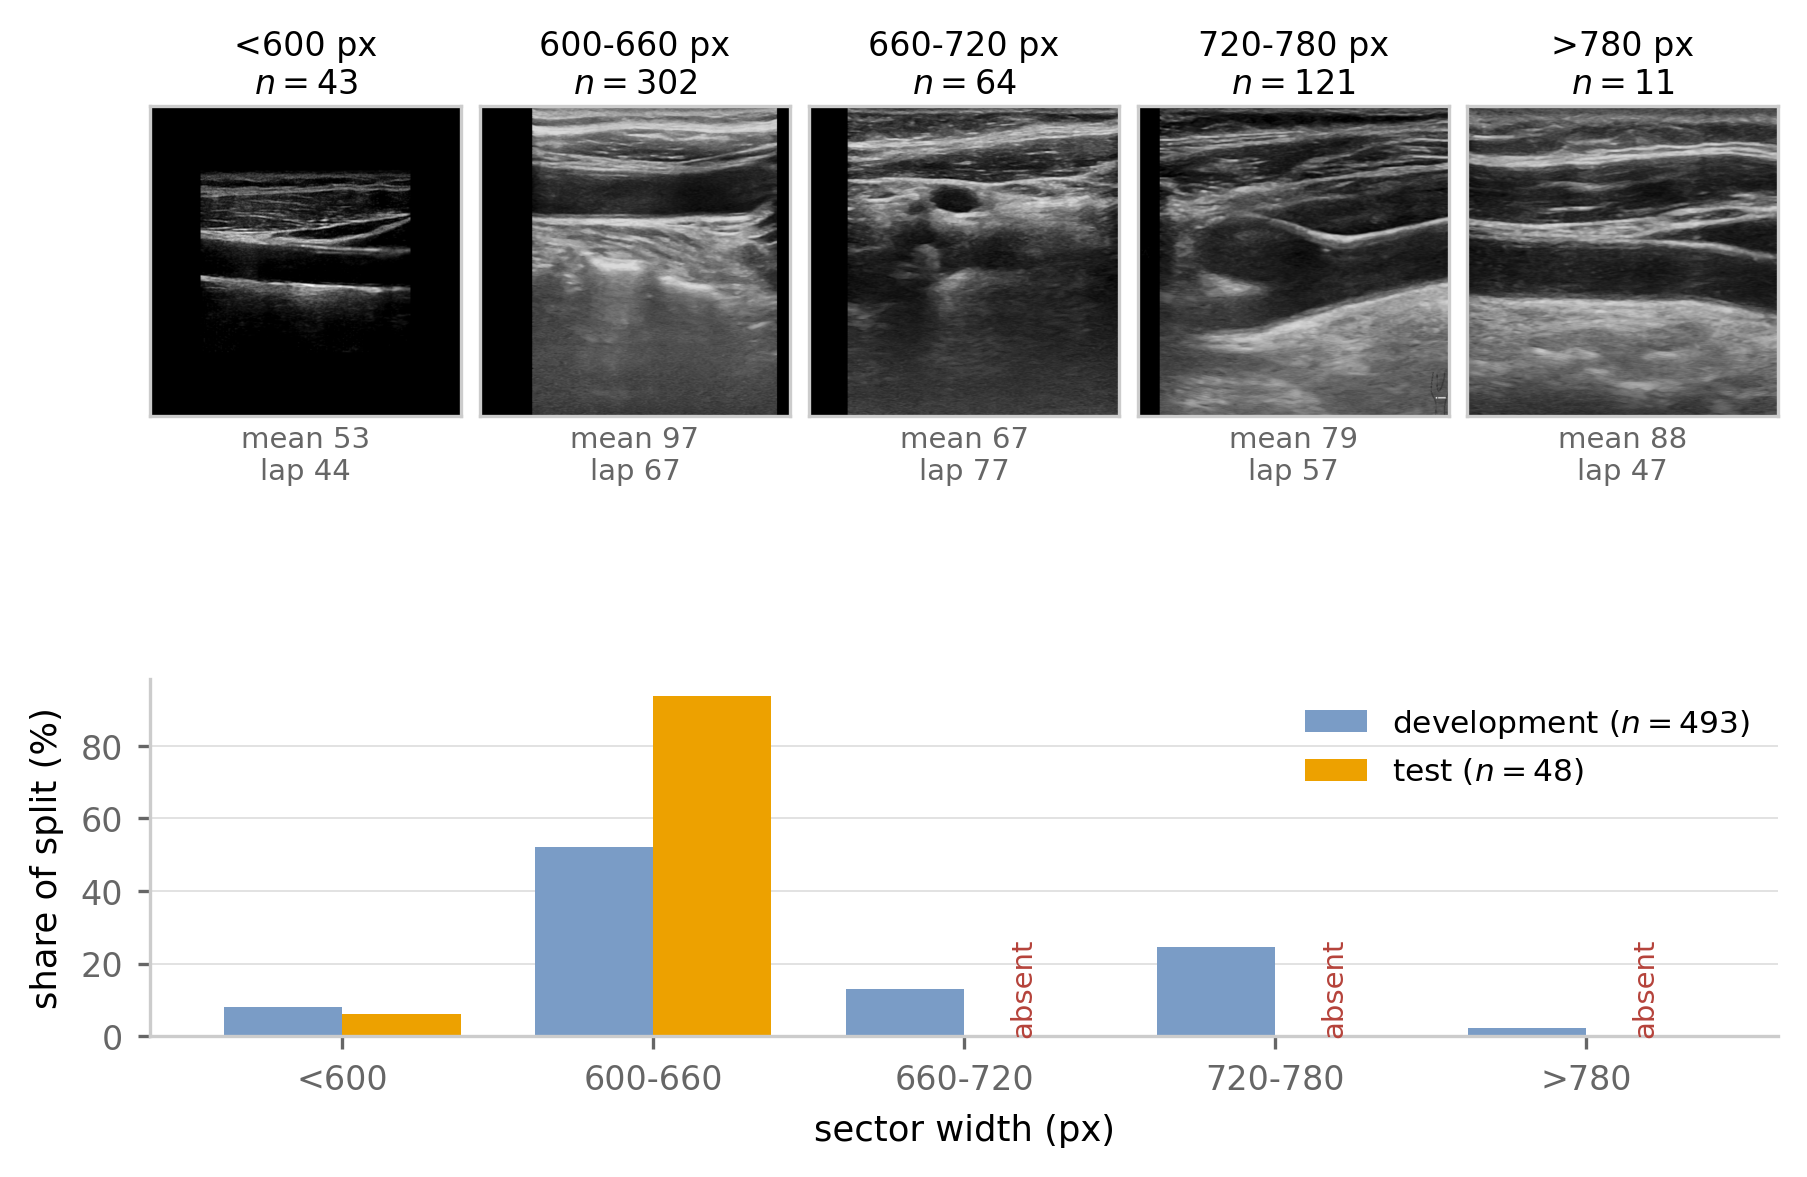
\includegraphics[width=\textwidth]{figures/acquisition_groups.png}
\caption[Acquisition heterogeneity in Ar-PlaqSegm1]{Top: a representative image from each
acquisition-geometry group, with the group's sector width, the number of images it contains, and
the median grey-scale intensity and Laplacian variance of that image. Bottom: the share of each
group in the development and test partitions. Three groups, comprising 196 of the 493 development
images, do not occur in the test partition at all.}
\label{fig:acquisition-groups}
\end{figure}

\subsubsection*{Duplicate images}
\label{subsec:duplicates}
The partition used throughout this thesis is the one distributed with the dataset; no image was
reassigned between training and test. Hashing the raw pixel data of the 541 images shows that
they comprise fewer distinct acquisitions than that number suggests: 26 groups of byte-identical
images occur, and four of these groups span both partitions of the published split, so four test
images are also present in the development partition. This overlap is a property of the dataset
as distributed rather than of any choice made here, and it applies to any evaluation that uses
the published partition without deduplicating it first. It was found by hashing the images before
training rather than inferred from the results. The consequences are quantified in
Section~\ref{sec:results-duplicates} and discussed in Section~\ref{sec:discussion-limitations},
and are deferred to there so as not to interrupt the description of the method.

\subsubsection*{Split}
The division into a development set of 493 pairs and a test set of 48 pairs is the one published
with the dataset and was adopted unchanged; it was not chosen for this thesis. The test set was
used exactly once per model, for the final evaluation reported in
Section~\ref{sec:results-phase2}. Its composition is balanced, with 24 plaque-positive and 24
plaque-negative images, while the development set contains 316 plaque-positive and 177
plaque-negative images. These counts reconcile exactly with the 340 and 201 reported for the
dataset as a whole.

The two partitions are not, however, comparable in composition. The test partition consists to
93.8\,\% of a single acquisition-geometry group, which accounts for only 52.1\,\% of the
development partition, and three of the five groups are absent from it entirely. The consequences
for the interpretation of the test results are discussed in
Section~\ref{sec:discussion-limitations}.
The dataset record does not state how many patients the 541 image pairs derive from, nor whether
the published split separates them at patient level. Image-level disjointness is verifiable and
holds apart from the duplicate groups reported above; patient-level disjointness is assumed, on
the grounds that a split constructed without it would be unusual, but it cannot be confirmed from
the material as distributed. If a patient did contribute images to both partitions, the test
figures of Chapter~\ref{ch:results} would be optimistic by an amount that cannot be estimated
here. The split is the dataset authors' own and was used unchanged, so this is a property of the
resource rather than a choice made in this work; it is recorded as a limitation in
Section~\ref{sec:discussion-limitations}.

Two properties make the dataset suitable for the purpose at hand. It originates from a different
country, imaging service and device generation, so the shift it represents is the one of
practical interest: whether a model developed on one cohort transfers to carotid ultrasound
acquired elsewhere. And its annotations are pixel-level masks rather than bounding boxes, which
permits the segmentation formulation examined in
Section~\ref{subsec:detection-to-segmentation}.

\subsection{External Validation of the Base Model}
\label{subsec:external-validation}
The base model was applied to the held-out test set to quantify the performance gap between its
development cohort and an external one. Its deployment pipeline preprocesses each image before inference: a fixed region-of-interest
crop, followed by median filtering and contrast-limited adaptive histogram equalisation. That
crop was defined for the UK Biobank image geometry and need not be appropriate for images
acquired with different devices and settings, where it may remove anatomy the model needs or
retain background it was never trained on. The model was therefore evaluated twice, once on
preprocessed and once on raw images, and the choice between the two variants was made on the
validation split rather than on the test set, for the reasons given in
Section~\ref{subsec:threshold-protocol}.

Evaluation is at the image level -- whether a plaque is detected anywhere in the image -- which is
the quantity the downstream cohort analyses consume, and which is directly comparable to the
image-level metrics reported for the base model in
Section~\ref{subsec:base-model-performance}.

\subsection{From Detection to Segmentation}
\label{subsec:detection-to-segmentation}
The annotations of the external dataset are pixel-accurate masks, whereas the base model is a
bounding-box detector. Carotid plaques are elongated structures that follow the curvature of the
vessel wall: across the 455 annotated plaque instances in the development set, the median aspect
ratio of the mask-derived bounding box is 4.6. A box drawn around such a structure consists
largely of non-plaque tissue, so the box representation discards most of what the annotation
encodes.

An instance segmentation model consumes the masks directly and, because a bounding box follows
from a predicted polygon at no additional cost, loses nothing that the detection formulation
provides. Fine-tuning was therefore carried out with segmentation models rather than detectors.
One trade-off is accepted: the warm start is a generic COCO-pretrained segmentation checkpoint
rather than the domain-specific model of \textcite{omarov2024deep}, which is detection-only and
cannot initialise a segmentation head. The domain knowledge is re-learned from the 455 annotated
polygons.

Two points follow for how the comparison in Chapter~\ref{ch:results} should be read. The first
is what is being compared. The base model is a detector trained on UK Biobank and applied to
Ar-PlaqSegm1 without adaptation; the fine-tuned models are segmentation models trained on the
Ar-PlaqSegm1 development set. They differ in two respects at once, the task they are trained on
and the data they are trained on, so a difference between them cannot be attributed to either
alone. A detection control, described in Section~\ref{subsec:detection-control}, was trained to
separate the two.

The second is what makes the comparison well defined despite the different outputs. Both
formulations produce instances carrying confidence scores, and the image-level decision --
whether a plaque is present anywhere in the image -- follows identically from both: an image is
positive if any instance exceeds the threshold. That decision is what the downstream cohort
analyses consume and is the quantity compared throughout. Mask quality, reported as the Dice
coefficient, is available only for the segmentation models, since the base model produces no
masks; no figure of that kind is compared across the two formulations.

\subsection{Dataset Construction}
\label{subsec:dataset-construction}
Each connected component of a mask was converted into one polygon instance. Components smaller
than 15 pixels were discarded as thresholding artefacts, and contours were simplified with the
Douglas-Peucker algorithm at a tolerance of 0.2\,\% of the contour arc length, which removes
near-collinear points without altering shape. Polygons with fewer than three remaining vertices
were dropped. The three representations are compared in Figure~\ref{fig:annotation-conversion}.
\begin{figure}[H]
\centering
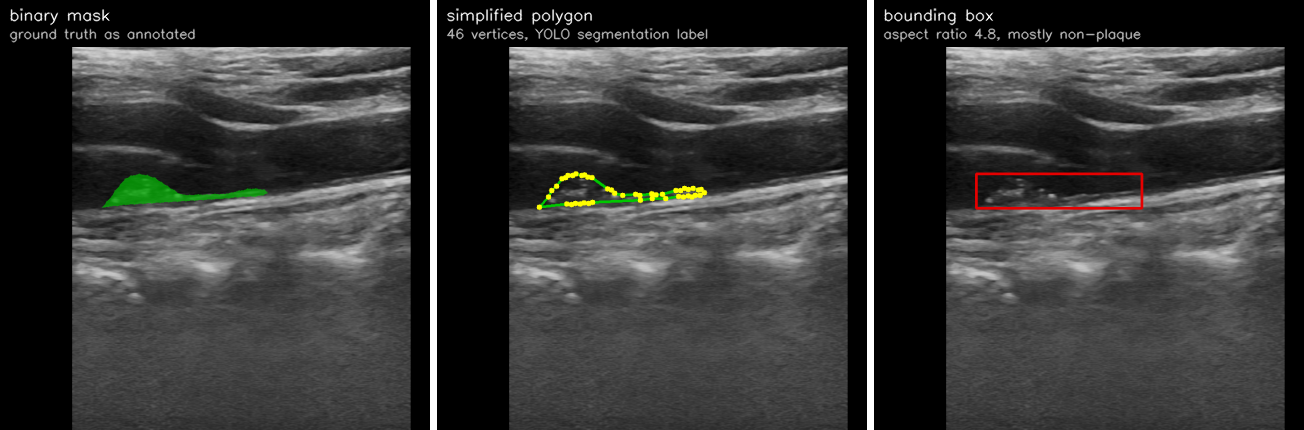
\includegraphics[width=\textwidth]{figures/annotation_conversion.png}
\caption[From mask to polygon to box]{The same annotation in three representations. Left: the
binary mask as provided with the dataset. Centre: the simplified polygon used as the
segmentation label, with its vertices marked. Right: the axis-aligned bounding box a detection
model would use instead. The box is what the detection formulation retains of the annotation.}
\label{fig:annotation-conversion}
\end{figure}
immediate rather than numerical.}
 Images annotated as plaque-free were retained with empty label files so that the
model also learns what not to detect.

The 493 development images were split into 420 training and 73 validation images, stratified by
plaque presence so that both splits retain a positive/negative mix, using a fixed random seed.
This yielded 385 polygon instances for training and 70 for validation.

\subsection{Model Training}
\label{subsec:model-training}
All models are YOLOv8 segmentation networks \cite{jocher2023ultralytics}, which extend the YOLOv8 detector
with a prototype-mask branch following the YOLACT principle \cite{bolya2019yolact}. A
\texttt{Proto} module produces 32 prototype masks at stride 4 from the highest-resolution feature
level, and each detected instance carries 32 coefficients whose linear combination, cropped to the
predicted box, forms its mask. Box regression uses distribution focal loss with 16 bins
\cite{li2020gfl}. Two model sizes were used: \texttt{yolov8m-seg} with 27{,}240{,}227
parameters and \texttt{yolov8s-seg} with 11{,}790{,}483.

Training started from COCO-pretrained checkpoints \cite{lin2014coco}, of which 411 of
417 tensors transfer; the six remaining are the class-dependent output layers, rebuilt for a
single class. Optimisation used AdamW at an initial learning rate of $10^{-3}$ decaying to
1\,\% of that value, with three warm-up epochs.

Augmentation was adapted to the modality. Vertical flipping was disabled because B-mode ultrasound
has a fixed anatomical orientation, with the probe at the top and depth increasing downwards, so a
vertical flip is physically impossible. Hue and saturation jitter were disabled because the images
are effectively greyscale, leaving brightness jitter as the only meaningful photometric variation.
Horizontal flipping (probability 0.5), rotation up to $5^\circ$, translation up to 10\,\%, scaling
up to 30\,\% and mosaic augmentation (probability 0.5) were retained.

From the second run onwards, copy-paste augmentation \cite{ghiasi2021copypaste} was enabled
at probability 0.3. This technique duplicates annotated instances into training images, so that
the model sees a greater number and variety of plaques per image than the annotations alone
provide; in the implementation used here the default mode pastes a horizontally mirrored copy of
an existing instance back into the same image. Because it operates on instance masks rather than
boxes, it is available only to the segmentation formulation and could not have been used for
detection training. It is the one segmentation-specific augmentation expected to help at this
dataset size, where 385 annotated polygons are available for training. Figure~\ref{fig:augmentation} shows one augmented batch.
\begin{figure}[H]
\centering
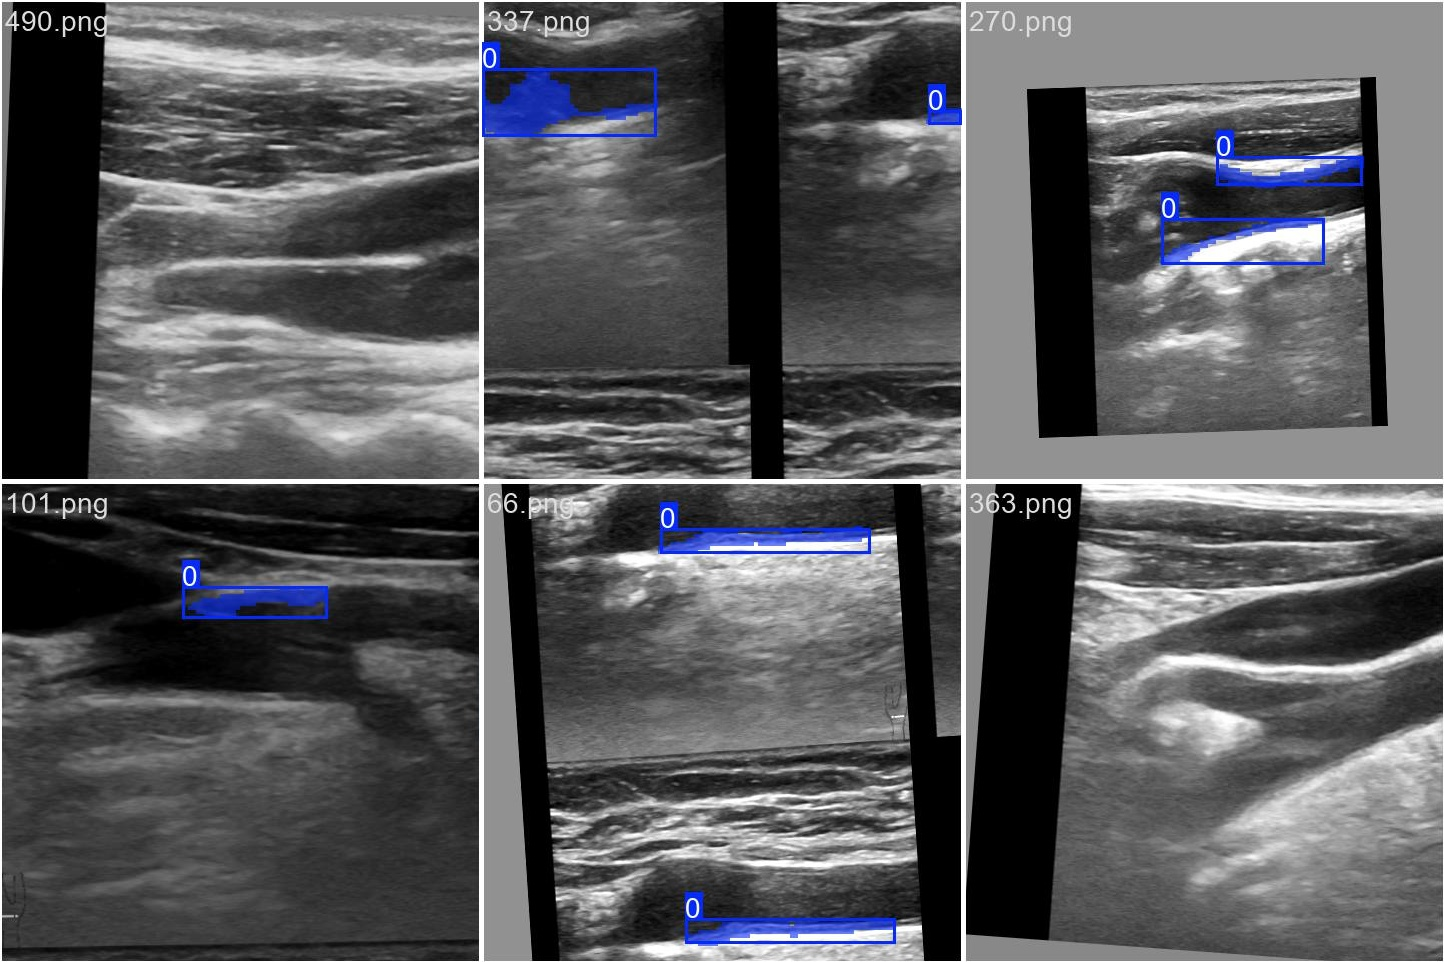
\includegraphics[width=0.85\textwidth]{figures/augmentation_batch.jpg}
\caption[An augmented training batch]{One training batch as presented to the network, written by
the training framework. Mosaic augmentation combines four images into one, and the geometric and
photometric transformations described above are applied on top; annotations are transformed with
the images.}
\label{fig:augmentation}
\end{figure}


Four models were trained (Table~\ref{tab:training-configs}). They differ in capacity, input
resolution and, from the second run onwards, in the classification loss weight. The rationale for
varying that weight is developed in Section~\ref{subsec:calibration-analysis}.

\begin{table}[H]
\centering
\caption[Training configurations]{Configurations of the four fine-tuned segmentation models. The
classification loss gain \texttt{cls} is varied systematically in the last three runs; all other
settings are held constant between them. ``Copy-paste'' denotes the instance-level augmentation
described above, which pastes mirrored copies of annotated plaques into the training images and
requires mask annotations.}
\label{tab:training-configs}
\begin{tabular}{llrrrrl}
\hline
Model & Checkpoint & Image size & Batch & Epochs & \texttt{cls} & Copy-paste \\
\hline
seg\_v1 & \texttt{yolov8m-seg} & 480 & 8  & 120 & 0.3 & no \\
seg\_v2 & \texttt{yolov8s-seg} & 640 & 16 & 226 & 0.3 & yes \\
seg\_v3 & \texttt{yolov8s-seg} & 640 & 16 & 250 & 1.0 & yes \\
seg\_v4 & \texttt{yolov8s-seg} & 640 & 16 & 250 & 0.5 & yes \\
\hline
\end{tabular}
\end{table}

Training used early stopping with a patience of 50 epochs; seg\_v2 stopped at epoch 226 of a
planned 300, while the remaining runs completed their full schedule.

All four runs were trained locally on an Apple M1 Pro with 16 GPU cores using the Metal
Performance Shaders backend. Training a single configuration to completion took approximately
5.2 hours at 250 epochs. This is distinct from the cohort-scale inference of
Section~\ref{sec:reproduction}, which ran on cloud infrastructure.

A note on the loss weighting is necessary because it becomes relevant to the results. In the
Ultralytics implementation the mask loss has no separate gain and is scaled by the box gain, so
the effective weighting of the four loss terms is 7.5 for the box loss, 7.5 for the mask loss, 1.5
for the distribution focal loss, and the value of \texttt{cls} for the classification loss. With a
single class, the classification branch is the confidence score. At the default of
\texttt{cls}~=~0.3 used in the first two runs, the term governing confidence was therefore
weighted twenty-five times lower than the terms governing geometry.

\subsection{Detection Control}
\label{subsec:detection-control}
To separate the change of formulation from the adaptation to the target domain, a bounding-box
detector was fine-tuned on the same material as the segmentation models. It used the same images,
the same split, the same schedule and the same hyperparameters as seg\_v2, with each polygon
annotation reduced to its enclosing box. It differs from seg\_v2 in its head and in the absence
of copy-paste augmentation, which operates on masks and cannot be applied to a box model. If the
segmentation formulation contributes beyond the adaptation, the detector should fall short of the
segmentation models at the image level; if it does not, the improvement over the base model is
attributable to the data rather than to the formulation. The outcome is reported in
Section~\ref{subsec:limitations-control}.

\subsection{Ensembling}
\label{subsec:ensembling}
Predictions from several models were combined by pooling. Each model is run independently at its
own training resolution, and the resulting instances are concatenated together with their
confidence scores; no averaging and no cross-model non-maximum suppression is applied. The usual
confidence threshold is then applied to the pooled set, so that an image counts as positive if any
instance from any model exceeds it, and the predicted mask is the union of the surviving
instances.

Suppression across models was deliberately avoided: for a single class it would discard precisely
those detections that only one model produced, which is the effect the pooling is intended to
exploit. The approach is motivated by the error analysis in
Section~\ref{subsec:results-error-analysis} and should be understood as a union of predictions,
not as a selection of the better one -- no information about the ground truth enters the
combination.

\subsection{Evaluation Metrics}
\label{subsec:metrics}
Three quantities are reported.

At the image level, sensitivity and specificity are computed from whether any instance exceeds the
confidence threshold, and summarised by Youden's~$J$ \cite{youden1950index}, defined as
sensitivity plus specificity minus one. This is the quantity the downstream cohort analyses
consume and the one directly comparable to the base model.

At the pixel level, agreement between the union of predicted masks and the ground-truth mask is
measured by the Dice coefficient \cite{dice1945measures}. Two aggregations are reported: the mean
over plaque-positive images, in which a missed plaque enters as zero rather than being excluded,
and a global coefficient pooling intersections and areas across the whole set, which is less
sensitive to individual small plaques.

At the instance level, mean average precision at an overlap threshold of 50\,\% (mAP@50) is
reported. A predicted instance counts as a true positive if its intersection over union with a
ground-truth instance reaches 0.5, precision and recall are evaluated across the full range of
confidence thresholds, and average precision is the area under the resulting precision-recall
curve; with a single class, the mean over classes is that value itself. The variant used here is
the mask form, in which the overlap is computed between predicted and annotated masks rather than
between boxes.

This quantity is reported for comparability with \textcite{omarov2024deep} and because the
training framework optimises against it, but it is not used to choose between models. It combines
two things this thesis separates -- whether a plaque is found at all, and how precisely it is
outlined -- and its overlap criterion is unforgiving for elongated structures, where a small
boundary error costs a disproportionate share of the intersection. Section~\ref{sec:results-phase2}
shows it diverging substantially from the image-level decision for the same models.

\subsection{Threshold Selection Protocol}
\label{subsec:threshold-protocol}
The confidence threshold is a free parameter, and choosing it on the test set would inflate the
reported performance even though no test image was trained on. All operating points reported in
this thesis are therefore selected on the validation split, by maximising Youden's~$J$ over a grid
in steps of 0.01, and then applied unchanged to the test set. For transparency, the value that
would have been obtained by optimising on the test set is reported alongside, so that the size of
the resulting optimism is visible rather than concealed.

This protocol is not fully independent: the validation split also selected the best checkpoint
during training. A strictly clean protocol would require a third split, which 493 annotated images
do not support. Choosing the threshold on validation is nonetheless substantially less circular
than choosing it on the test set.

\subsection{Error Analysis}
\label{subsec:calibration-analysis}
Two diagnostic analyses were performed beyond the headline metrics.

Confidence scores produced by modern neural networks are known to be poorly calibrated
\cite{guo2017calibration}, and two analyses were run to establish whether that is what limits
the models here.

The first isolates the contribution of confidence ranking. For each plaque-positive test image,
the best-matching predicted instance is identified irrespective of its confidence score, and the
Dice coefficient of that instance is recorded. Comparing this quantity with the Dice obtained at
the operating threshold separates two failure modes that the headline metrics conflate: a model
that does not produce a correct mask at all, and a model that produces one but ranks it below the
threshold. The median confidence carried by these best-matching instances quantifies how severely
the confidence scale is misplaced.

The second tests whether the ranking can be repaired after training. A logistic regression was
fitted on the validation split to re-score each predicted instance from features available at
inference time -- the original confidence on a logarithmic scale, mask area, aspect ratio, fill
ratio, vertical position, local echo contrast against a surrounding ring, intensity variation
within the mask, and the instance's rank and count within its image. Generalisation was estimated
by five-fold cross-validation grouped by image, since instances from the same image are strongly
correlated. The re-scored values then replaced the confidences and the standard evaluation was
repeated. Because the two scores occupy different scales, the comparison was made across matched
quantiles of each score distribution rather than at a shared absolute threshold.

Monotone recalibration methods such as Platt scaling \cite{platt1999probabilistic} or isotonic regression
\cite{zadrozny2002transforming} were not applicable: they rescale confidences while preserving
their order, and Section~\ref{subsec:results-calibration} shows the order to be the defective
property.
